\chapter{Magnetismo de sólidos} \label{Ch:10}

En este Capítulo se estudian algunas de las contribuciones más importantes al magnetismo de los sólidos. Como se verá, alguna de ellas (como la ferromagnética) constituye un fenómeno cooperativo que lleva asociado una transición de fase. Es también destacable que el magnetismo de sólidos es en buena medida un efecto cuántico dado que muchas de sus causas (el momento mangnético de espín, la interacción de intercambio, etc.) no tienen análogo clásico.

\section{Relaciones básicas}

\section{Diamagnetismo atómico}

\section{Paramagnetismo atómico}

\subsection{Origen del momento mangnético atómico}

\subsection[Dependencia de la magnetización respecto $\vec{\Bn}$ y $T$]{Dependencia de la magneteización paramagnética con la temperatura y el campo magnético}

\subsection{Ley de Curie}

\section{Paramagnetismo de los electrones de conducción}

\section{La interacción de intercambio}

\section{Ferromagnetismo}

\section{Dominios ferromagnéticos}

\section{Orden ferrimangnético}

\begin{figure}[h!] \centering
	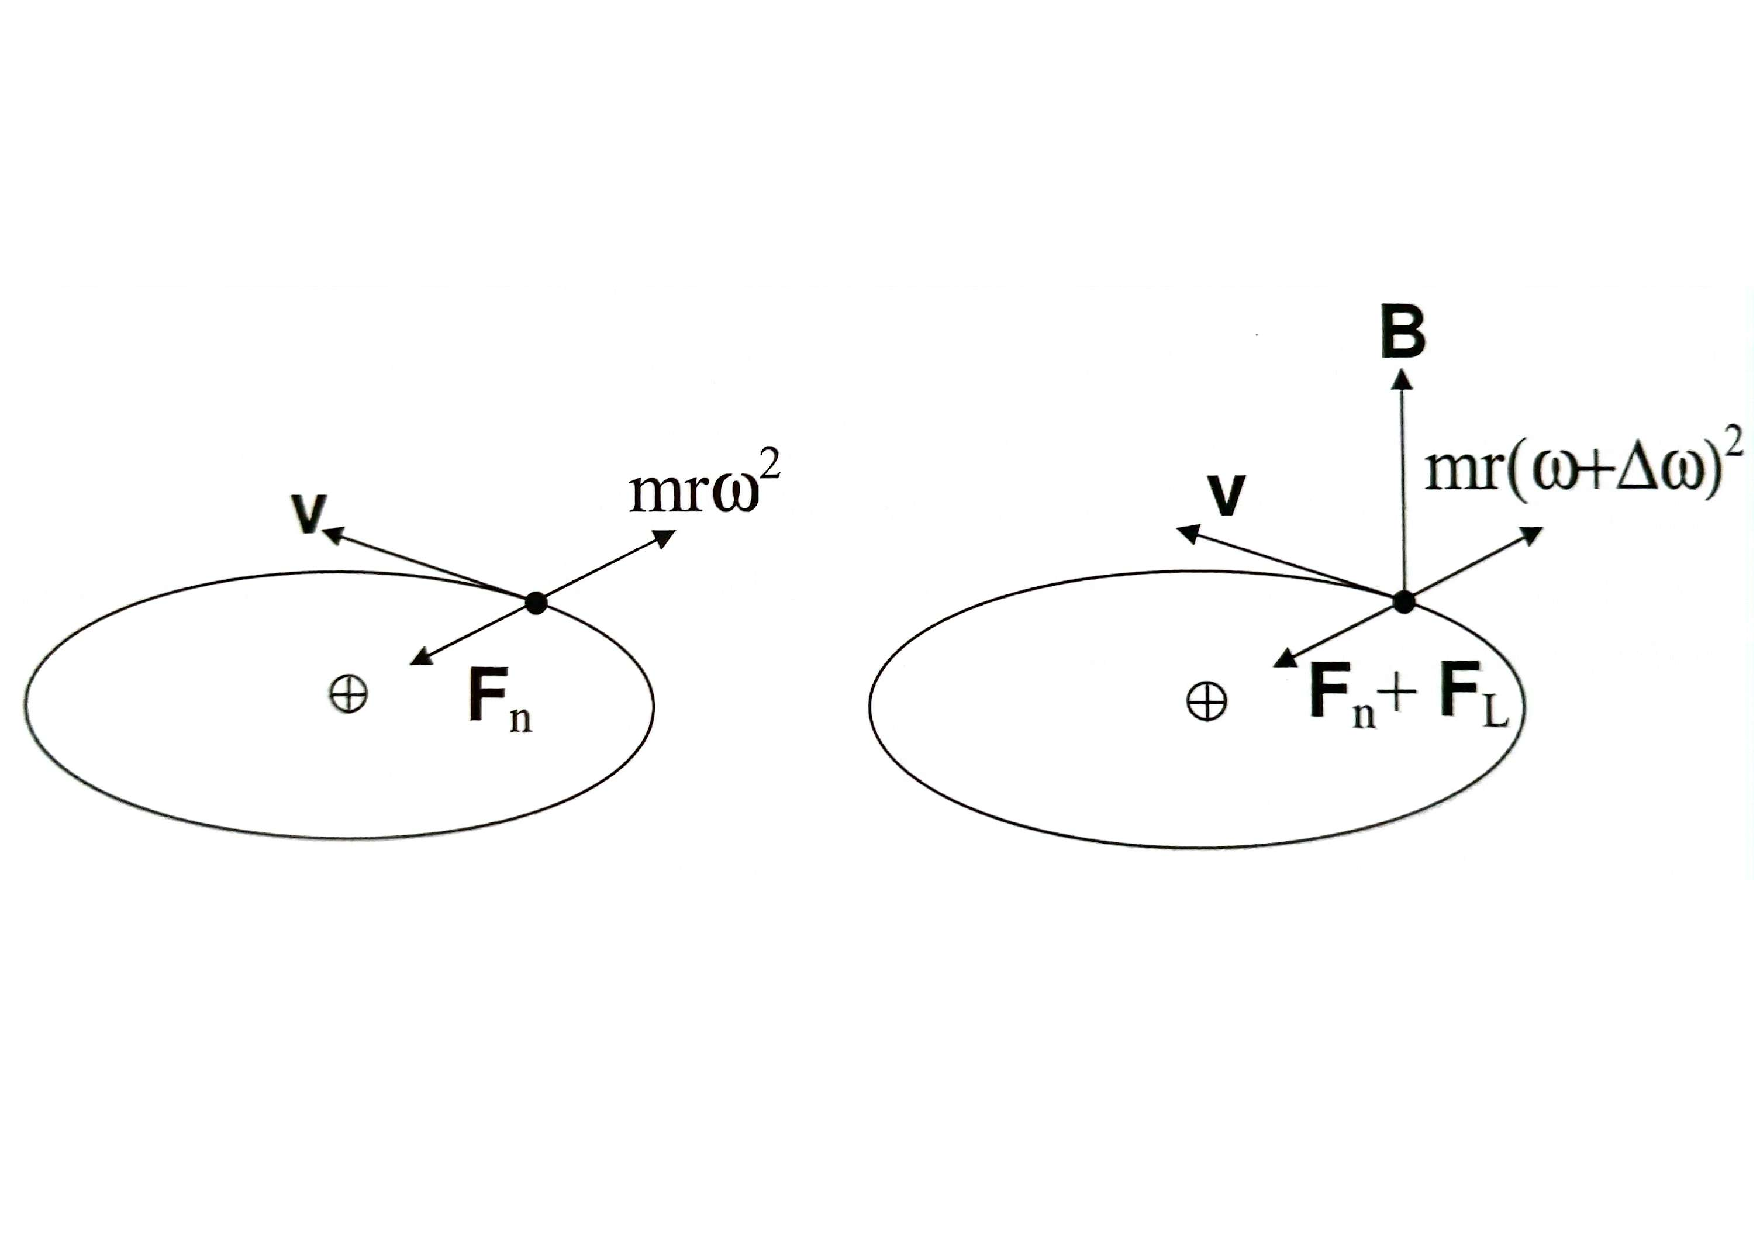
\includegraphics[scale=0.5]{Cuerpo/Ch_10/Fotos libro 1.pdf}
	\caption{}
	\label{Fig:10-01}
\end{figure}
\begin{figure}[h!] \centering
	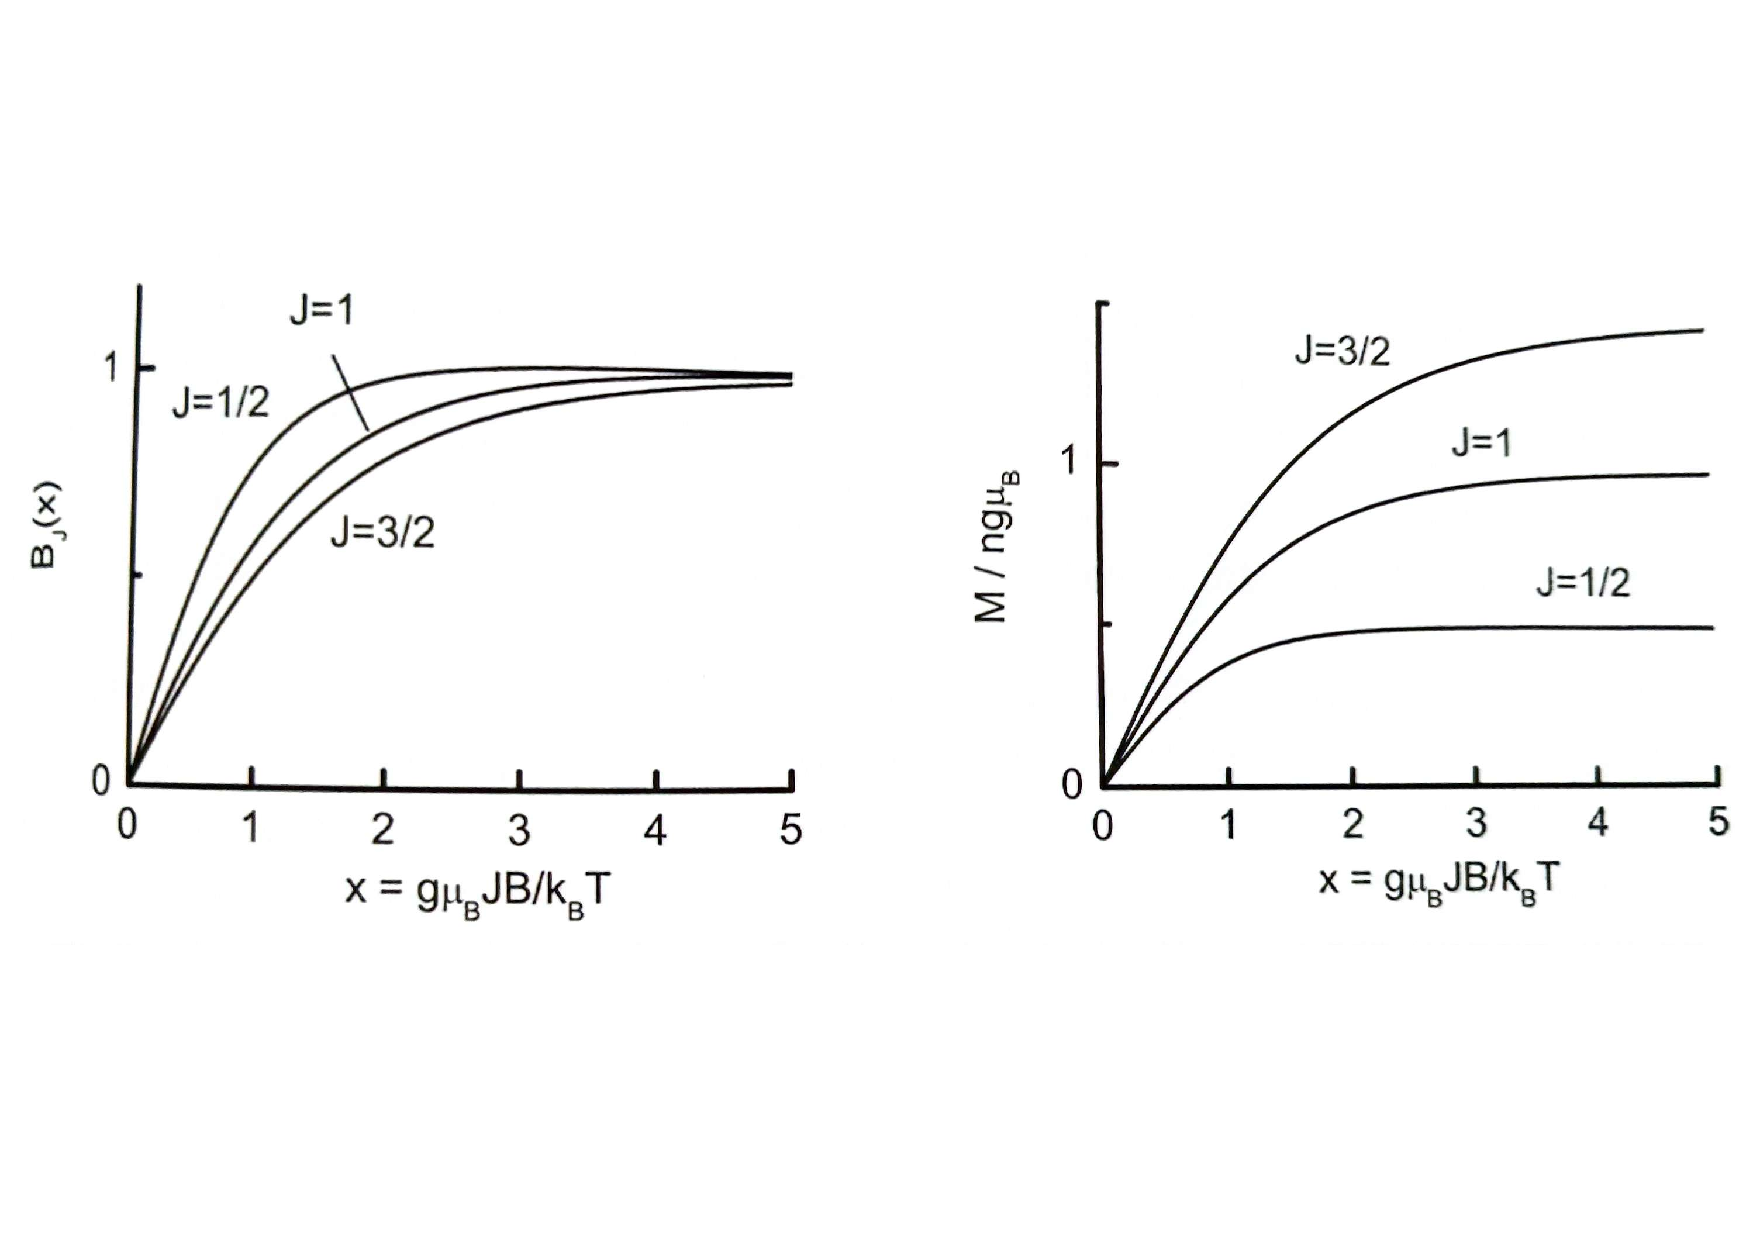
\includegraphics[scale=0.5]{Cuerpo/Ch_10/Fotos libro 2.pdf}
	\caption{}
	\label{Fig:10-02}
\end{figure}
\begin{figure}[h!] \centering
	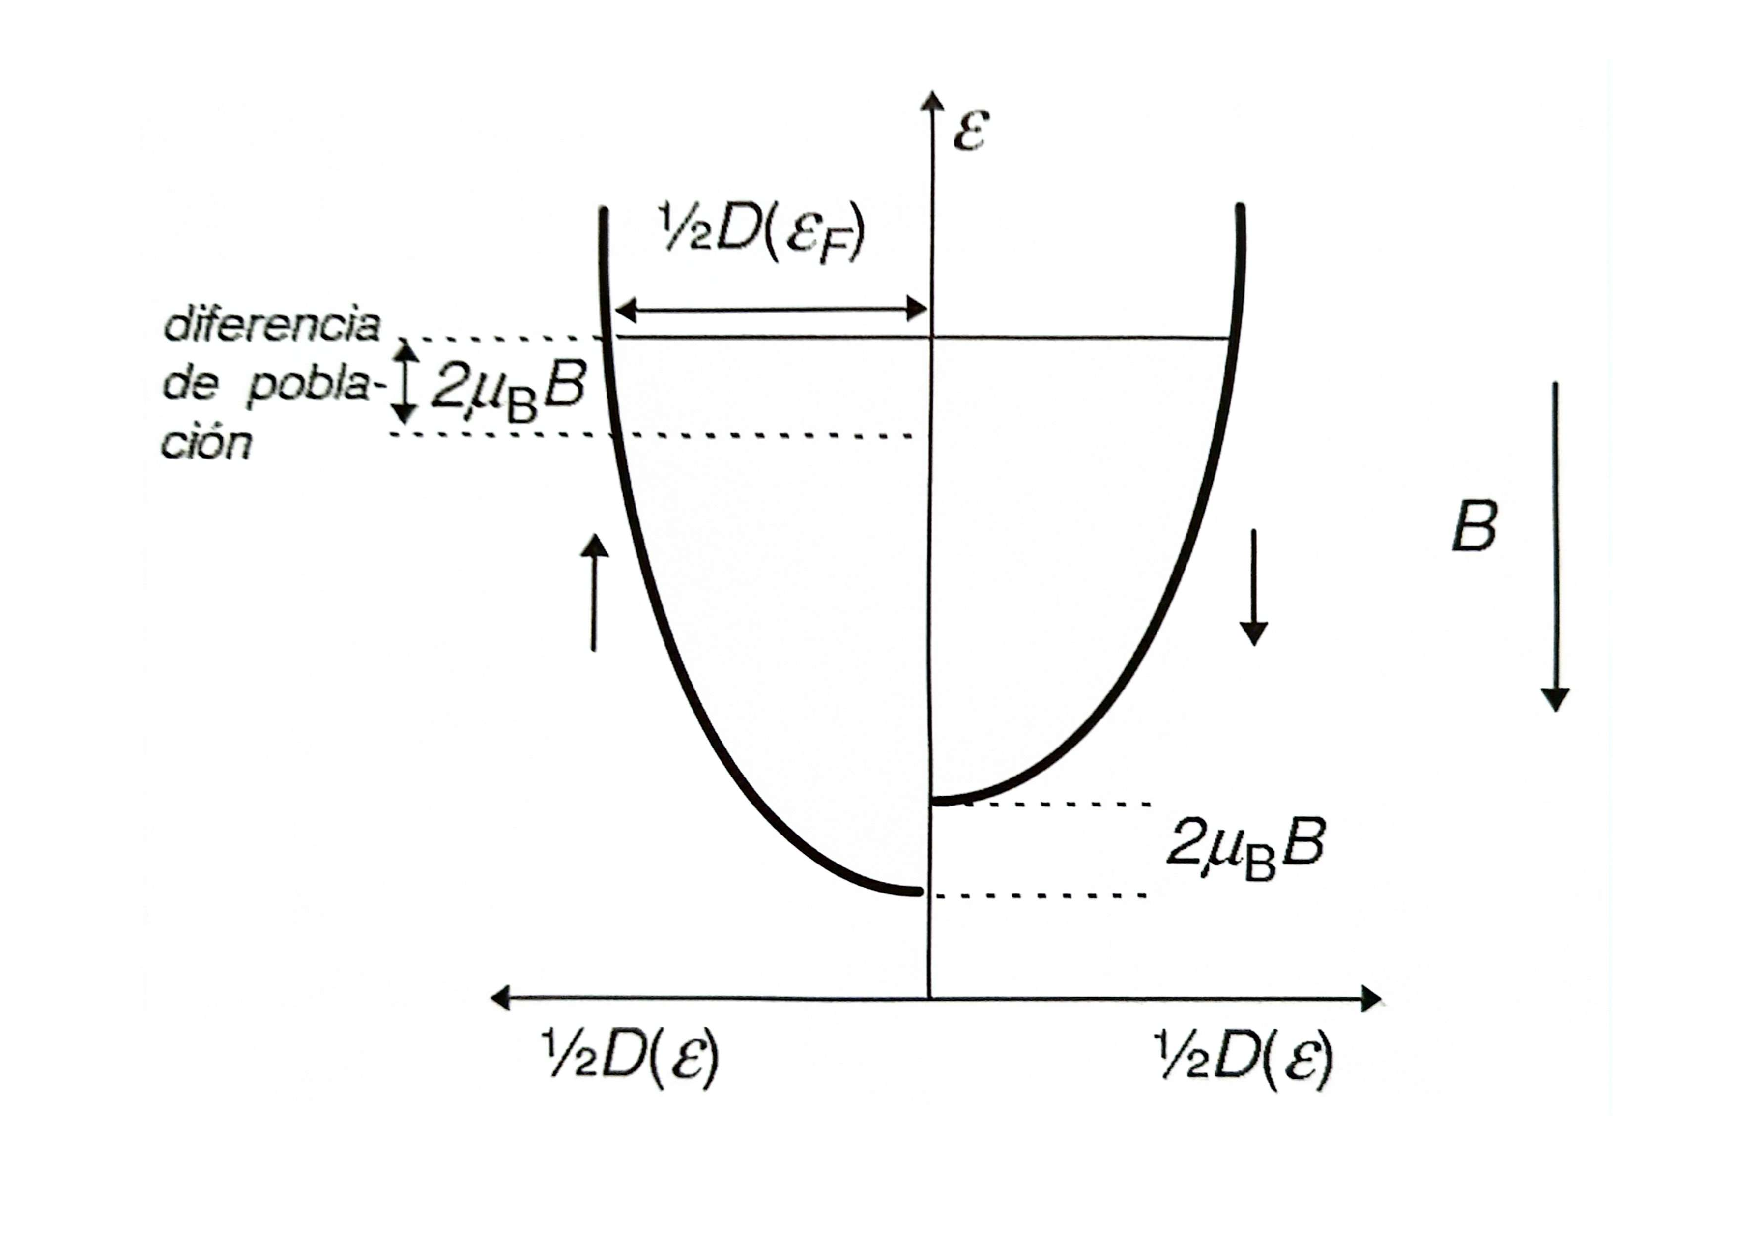
\includegraphics[scale=0.5]{Cuerpo/Ch_10/Fotos libro 3.pdf}
	\caption{}
	\label{Fig:10-03}
\end{figure}
\begin{figure}[h!] \centering
	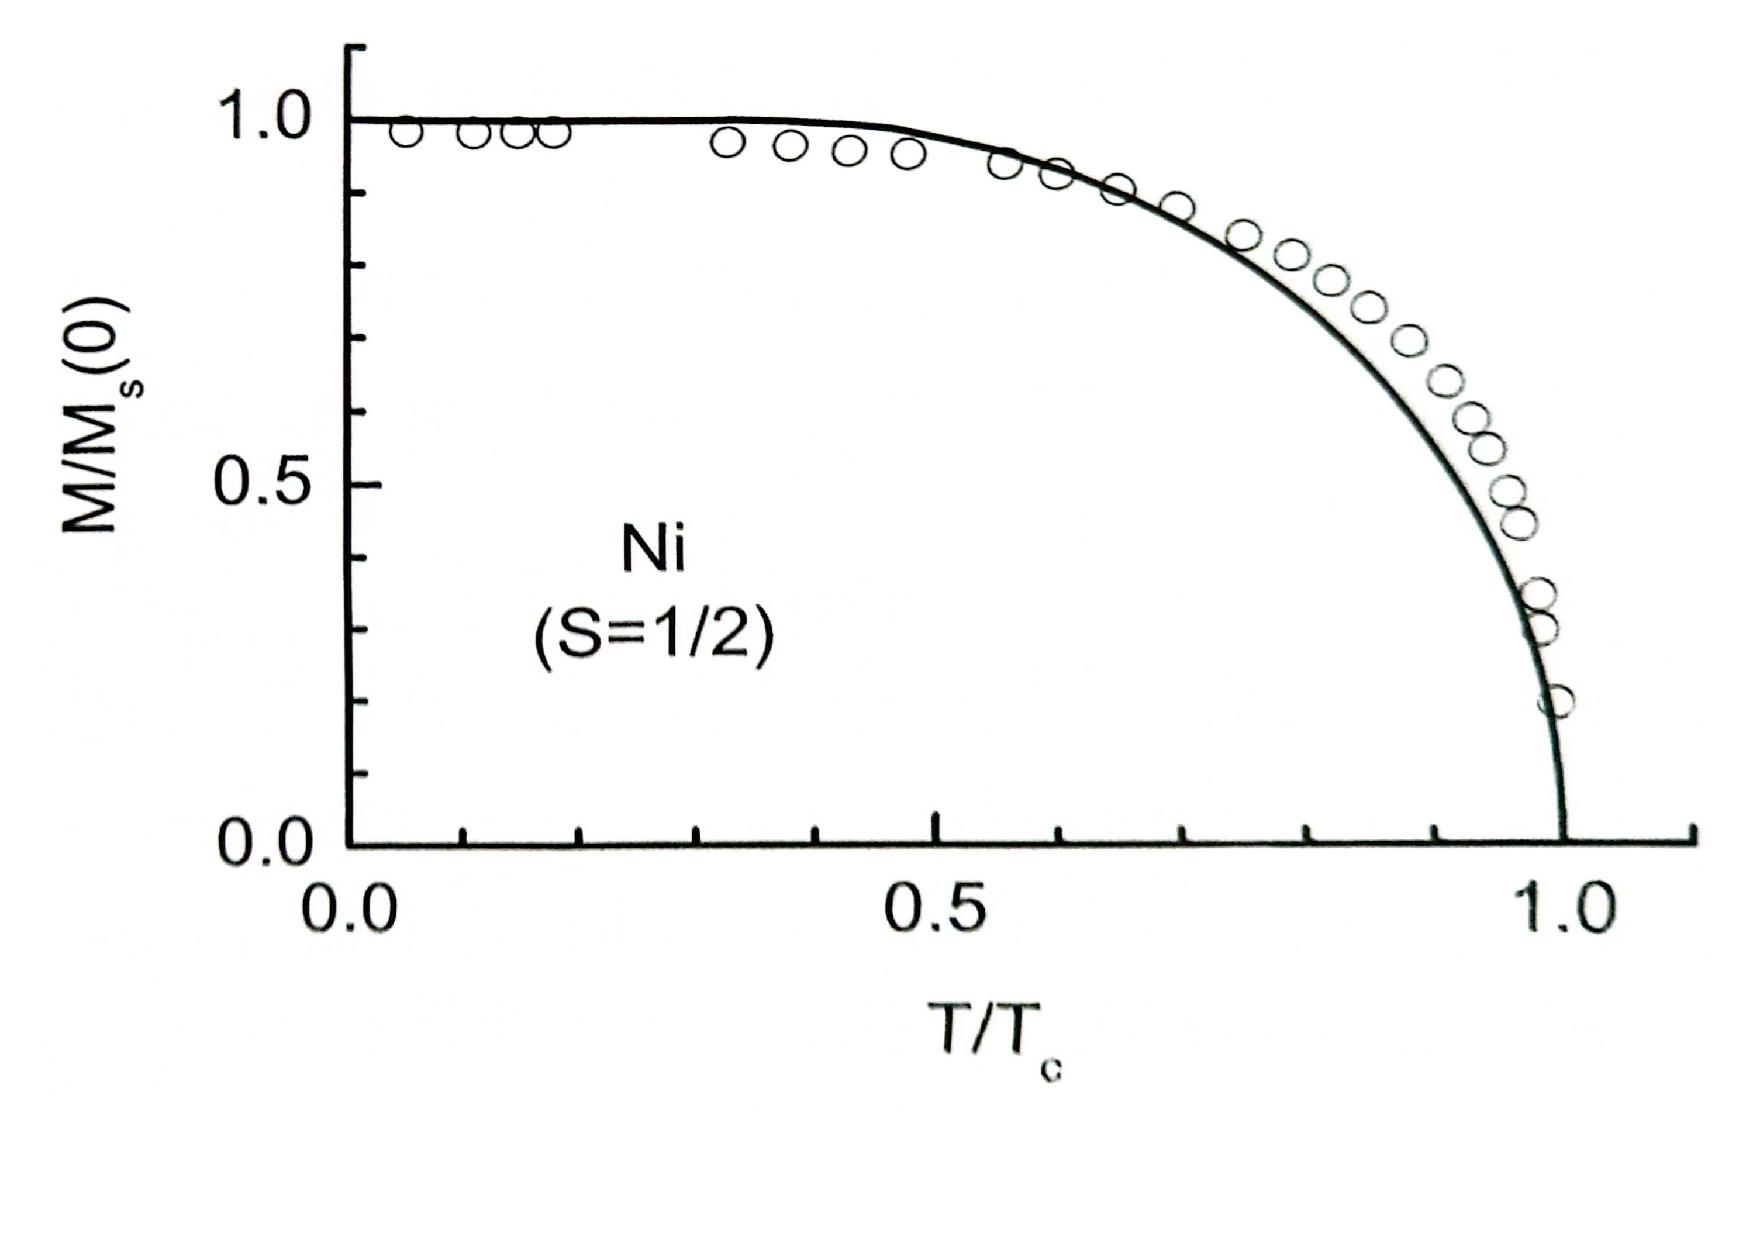
\includegraphics[scale=0.5]{Cuerpo/Ch_10/Fotos libro 4.pdf}
	\caption{}
	\label{Fig:10-04}
\end{figure}
\begin{figure}[h!] \centering
	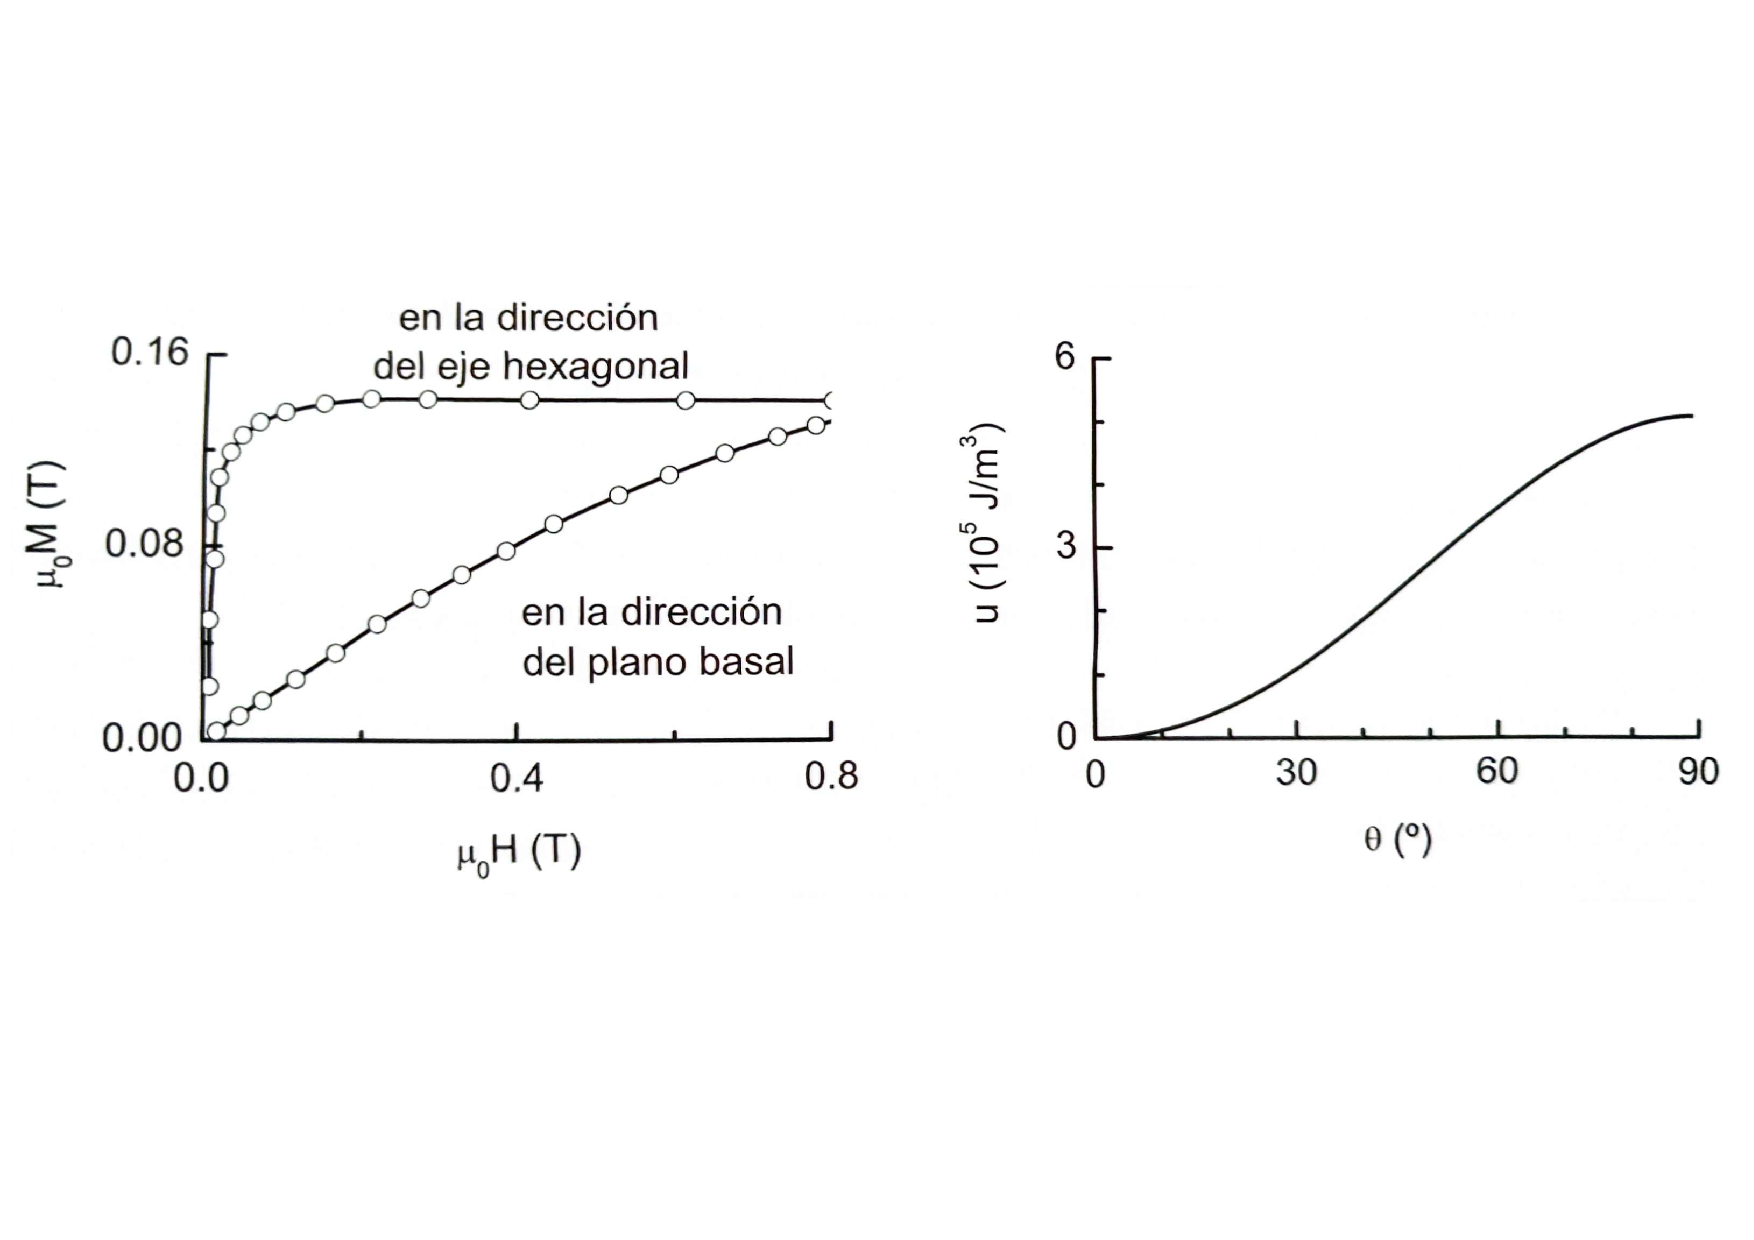
\includegraphics[scale=0.5]{Cuerpo/Ch_10/Fotos libro 5.pdf}
	\caption{}
	\label{Fig:10-05}
\end{figure}
\begin{figure}[h!] \centering
	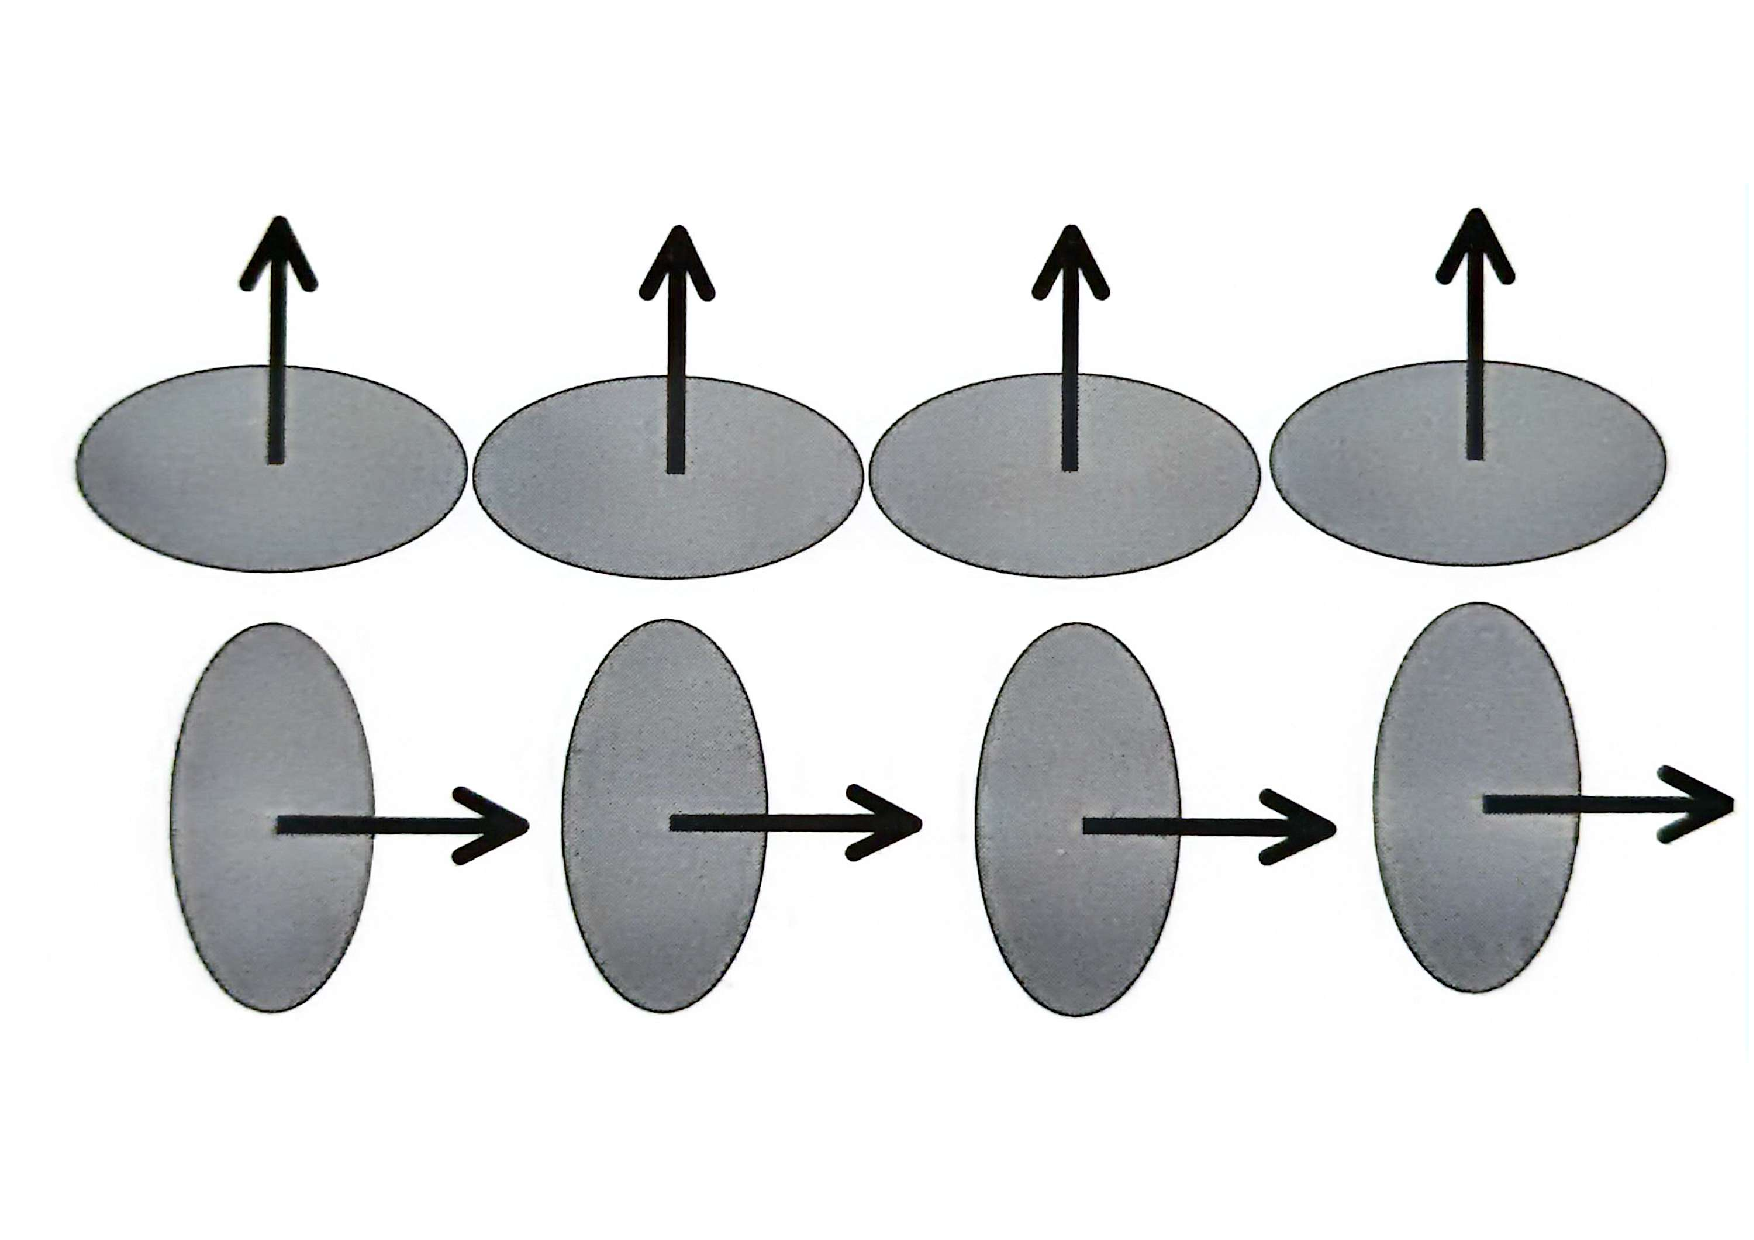
\includegraphics[scale=0.5]{Cuerpo/Ch_10/Fotos libro 6.pdf}
	\caption{}
	\label{Fig:10-06}
\end{figure}
\begin{figure}[h!] \centering
	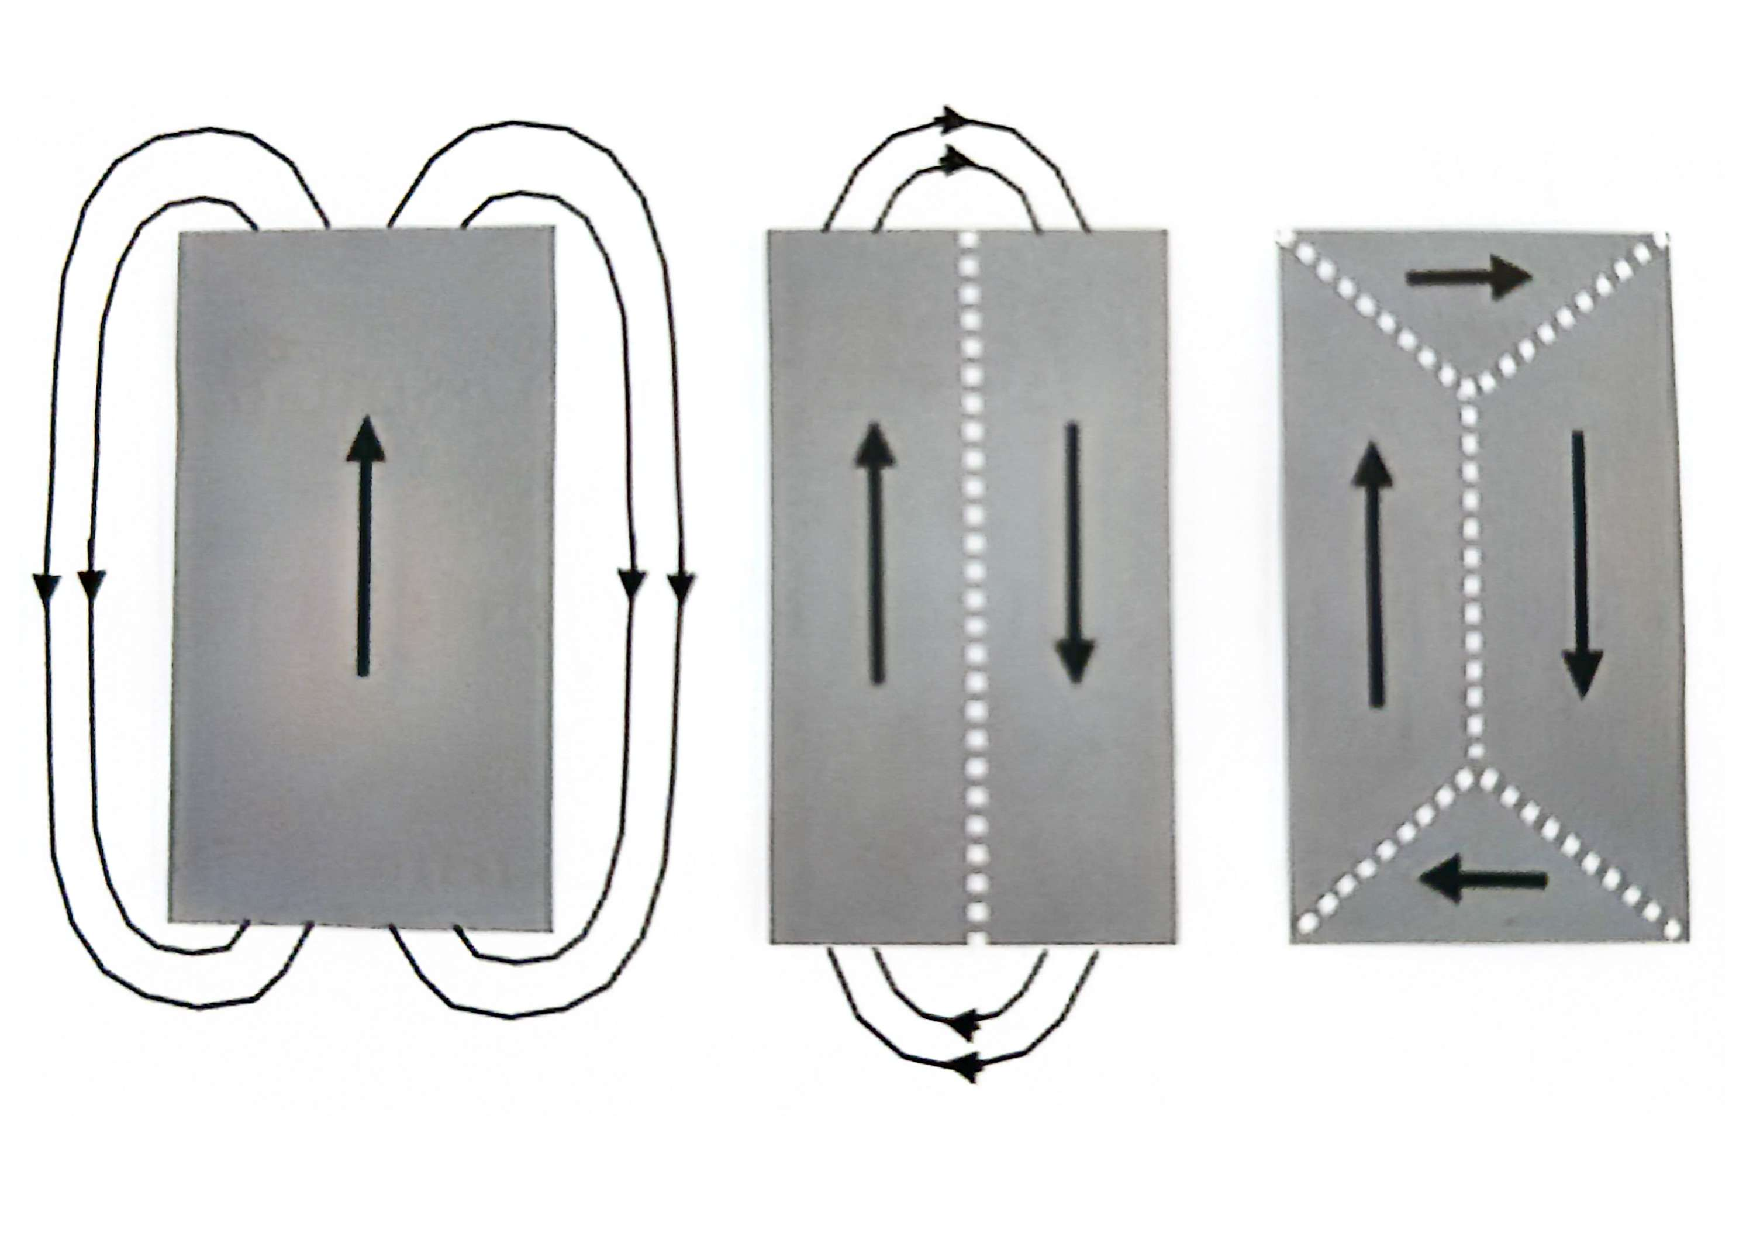
\includegraphics[scale=0.5]{Cuerpo/Ch_10/Fotos libro 7.pdf}
	\caption{}
	\label{Fig:10-07}
\end{figure}
\begin{figure}[h!] \centering
	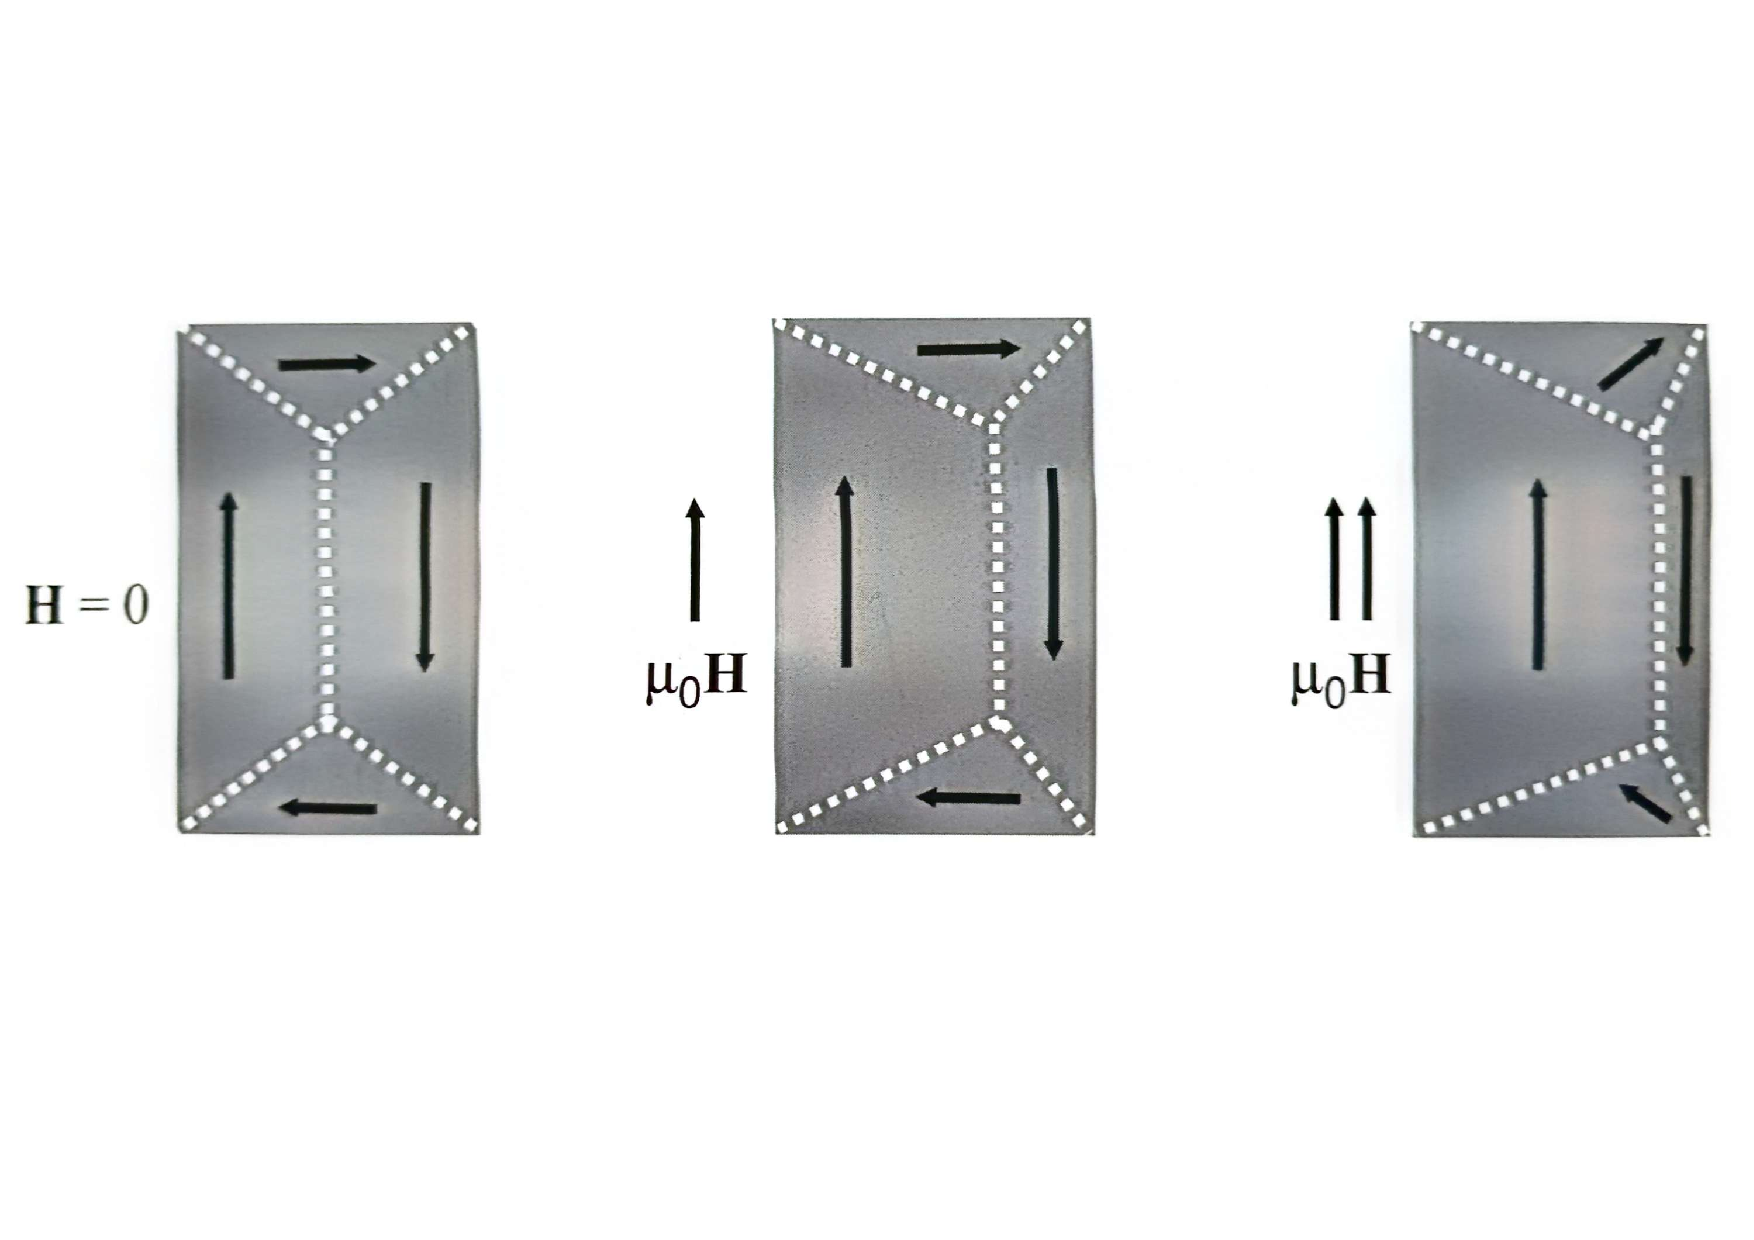
\includegraphics[scale=0.5]{Cuerpo/Ch_10/Fotos libro 8.pdf}
	\caption{}
	\label{Fig:10-08}
\end{figure}
\begin{figure}[h!] \centering
	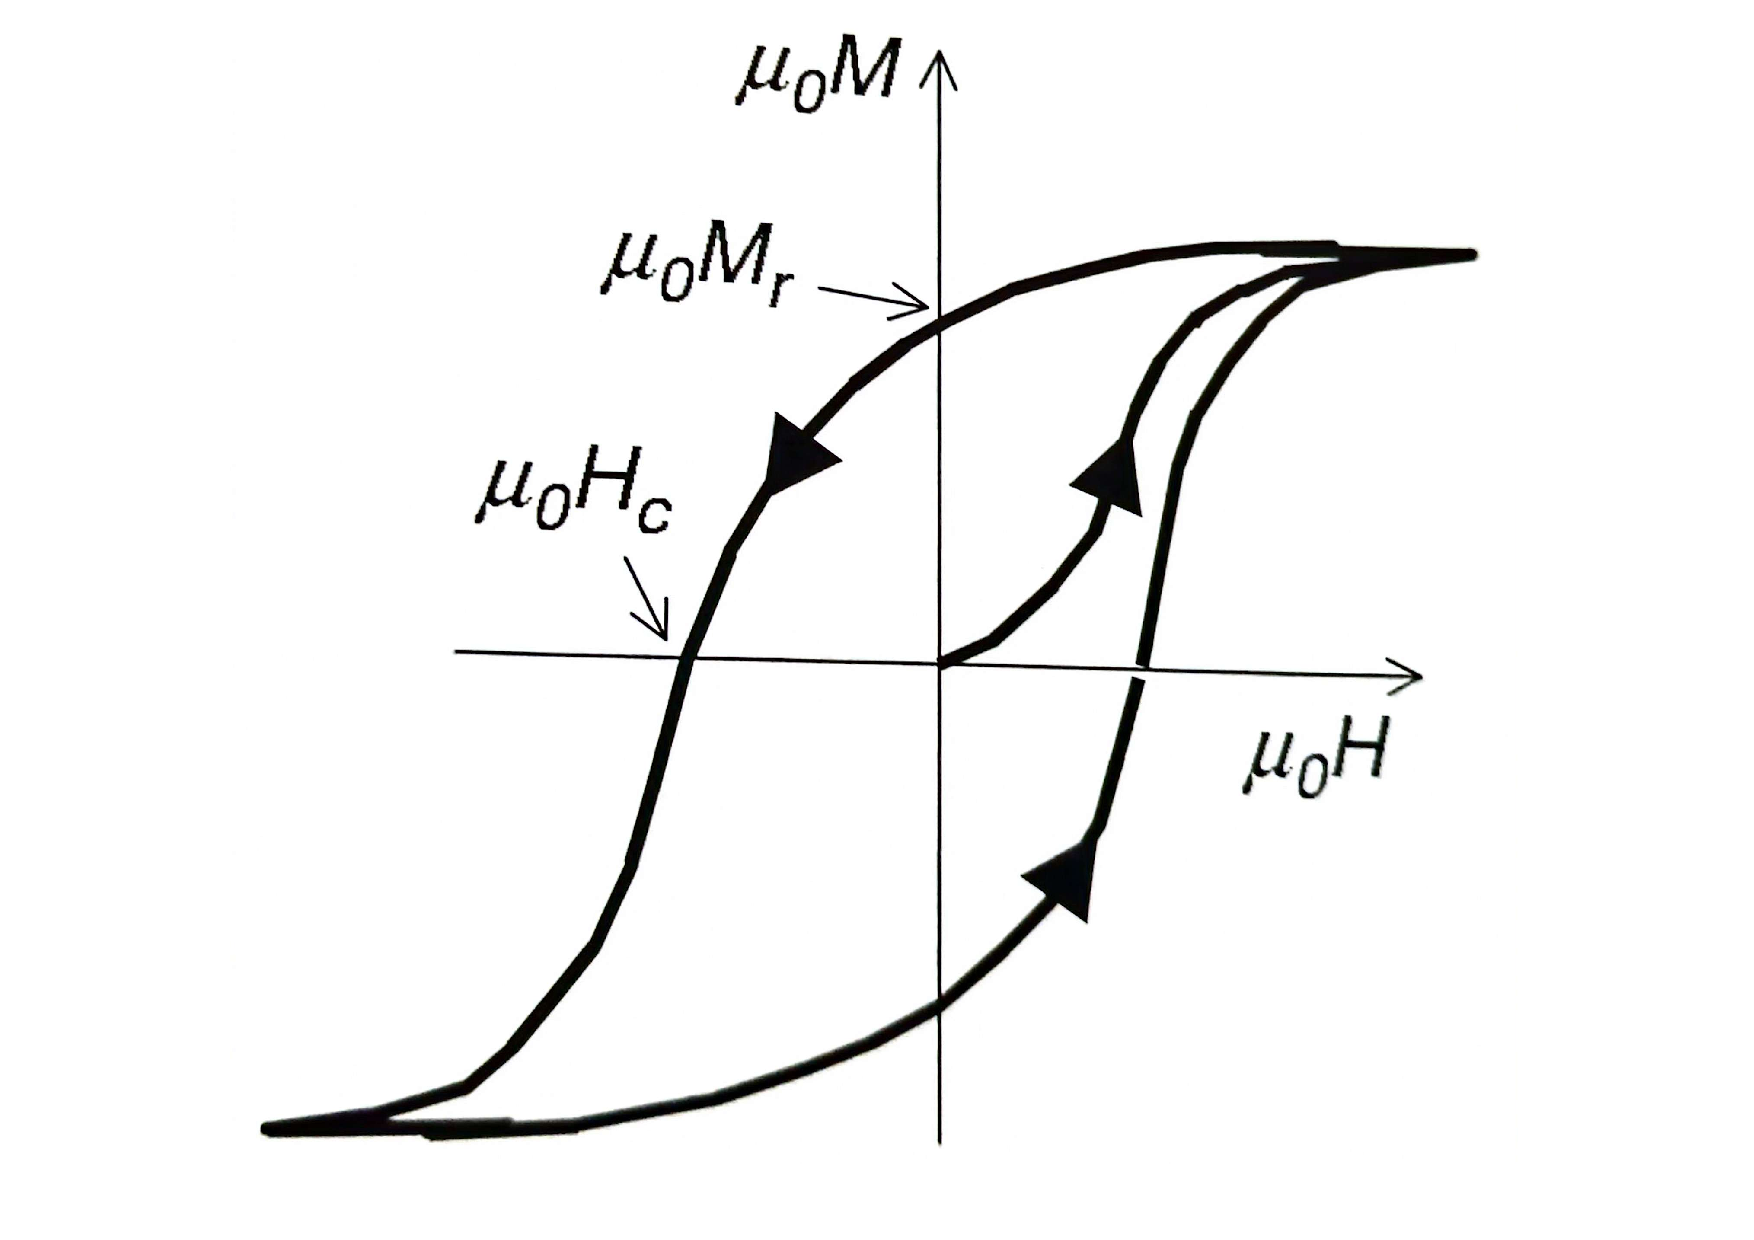
\includegraphics[scale=0.5]{Cuerpo/Ch_10/Fotos libro 9.pdf}
	\caption{}
	\label{Fig:10-09}
\end{figure}